\begin{frame}{Manufacturing Process}
    \begin{center}
        \begin{tikzpicture}%[x=1cm, y=1cm]
        
        \node[visible on=<1->, arrow] at (1.1,5.9) (fab) {Fab};
        \node[visible on=<2->, arrow, right=\arrow of fab] (sort)  {Sort};
        \node[visible on=<3->, arrow, right=\arrow of sort]  (die_bank) {Die bank};
        \node[visible on=<4->, arrow, right=\arrow of die_bank] (assemble)  {Assemble};        
        \node[visible on=<5->, arrow, right=\arrow of assemble] (test) {Test};
        \node[visible on=<6->, finalblock, right=\arrow of test] (dc) {Distribution};	
                
        % Semiconductor manufacturing process graphics
        \node[visible on=<1->, above=\y of fab] (fab_img) {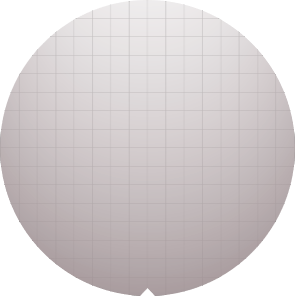
\includegraphics[scale=0.3]{structured_wafer.png}};
        \node[visible on=<2->, above=\y of sort] (sort_img) {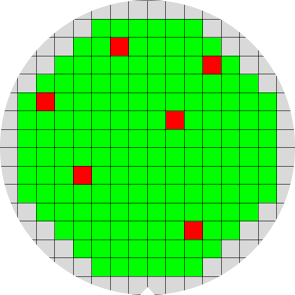
\includegraphics[scale=0.3]{sort.png}};
        \node[visible on=<3->, above=\y of die_bank] (die_bank_img) {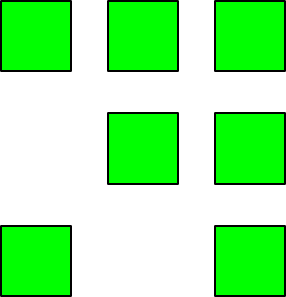
\includegraphics[scale=0.23]{die_bank.png}};
        \node[visible on=<4->, above=\y of assemble] (assembly_img) {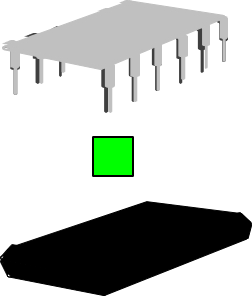
\includegraphics[scale=0.3]{assembly.png}};
        \node[visible on=<5->, above=\y of test] (test_img) {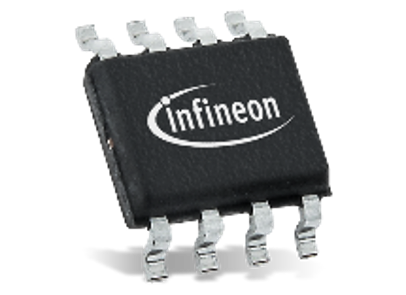
\includegraphics[scale=0.3]{test.png}};
        \node[visible on=<6->, above=\y of dc] (dc_img) {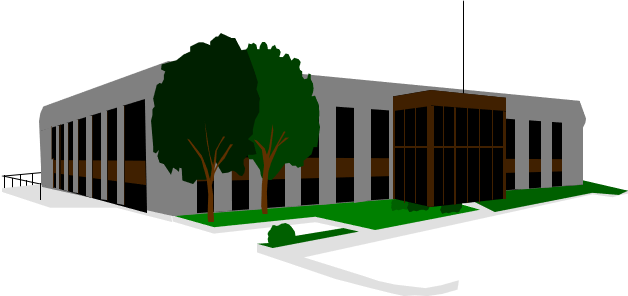
\includegraphics[scale=0.24]{distribution.png}};
        
        \end{tikzpicture}
    \end{center}
\end{frame}

\begin{frame}{Scanning Electron Microscope}
\begin{figure}
    \hspace{15mm}
        \begin{tikzpicture}
          \draw[gray,fill=gray,path fading=south] (0,0) rectangle +(5,-2);% sample
            \begin{scope}[decoration={snake,amplitude=.4mm,
                segment length=2mm,post length=1mm}]
              \draw[decorate,blue,->] (2.5,0) -- ++(112:3);% x-ray
              \draw[decorate,red,->] (2.5,0) -- ++(5:2);% auger
              \draw[decorate,orange,->] (2.5,0) -- ++(45:3);% cathodlimuescence
            \end{scope}
          \fill[color=red, path fading=north,fading transform={rotate=-15}]
            (2.5,0) ++(60:3) ++(150:0.1) -- ++(-30:0.2) -- (2.5,0) -- cycle;%backscatter
          \fill[color=green, path fading=north,fading transform={rotate=45}]
            (2.5,0) ++(135:2) ++(225:0.3) -- ++(45:0.6) -- (2.5,0) -- cycle;%secondary
          \shade[inner color=blue, top color=blue] (2.2,1.8)
            -- ++(0.6,0) -- ++(-0.3,-1.8) -- cycle;%primary occhelectrons
        
          \shade[left color=gray!50!white,right color=gray] (1.7,3)
            -- ++(1.6,0) -- ++(-0.3,-1) -- ++(-1,0) -- cycle;% column
          \shade[left color=gray!50!white,right color=gray] (2.1,2)
            -- ++(0.8,0) -- ++(0,-0.2) -- ++(-0.8,0) -- cycle;% column bottom
          \draw[gray!80!black] (1.7,3) -- ++(1.6,0) -- ++(-0.3,-1)
            -- ++(-1,0) -- cycle;%column
          \draw[gray!80!black] (2.1,2) -- ++(0,-0.2) -- ++(0.8,0)
            -- ++(0,0.2);%column bottom
        		
          \shade[left color=gray!50!white,right color=gray] (2.5,0) ++(135:2) --
            ++(225:0.3) -- ++(135:0.8) -- ++(45:0.6) -- ++(315:0.8) -- cycle;% detector
        		
          %labels
          \draw (0,-2) node[above right] {\footnotesize Observed sample};
          \draw (2.5,0) ++(5:2) node[right] {\footnotesize Auger};
          \draw (2.5,0) ++(45:3) node[right] {\footnotesize Cathodeluminescence};
          \draw (2.5,0) ++(60:3) node[right] {\footnotesize Backscattered};
          \draw (2.5,0) ++(112:3) node[left] {\footnotesize X-ray};
          \draw (2.5,0) ++(135:1.2) node[left=0.4cm] {\footnotesize Secondary};
          \draw (2.5,0) ++(135:2) ++(225:0.3) ++(135:0.8) node[left]
            {\footnotesize Detector};
        \end{tikzpicture}
        \caption*{Scanning electron microscope (SEM).}
\end{figure}    
\end{frame}

\begin{frame}{SEM Inspection}
    \begin{center}
        \begin{tikzpicture}
            % Fab process flow at the bottom of the figure
            \node[visible on=<1->, inner sep=0mm] (raw_wafer_img) at (1.1,1.75) {
\includegraphics[scale=0.17]{raw_wafer.png}};
            \node[visible on=<1->, step_rectangle, right=\step of raw_wafer_img] (step1)  {Step 1};
            \node[visible on=<1->, step_rectangle, right=\step of step1] (step2)  {Step 2};
            \node[visible on=<1->, step_rectangle, right=\step of step2] (step3)  {\ldots};
            \node[visible on=<1->, step_rectangle, right=\step of step3] (stepn)  {Step n};
            \node[visible on=<1->, inner sep=0mm, right=\step of stepn] (wafer_img) {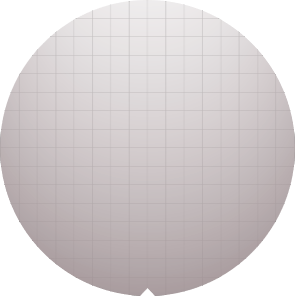
\includegraphics[scale=0.17]{structured_wafer.png}};
            
            % Arrows lining the fab process flow at the bottom of the figure
            \draw[visible on=<1->, arrow_small] (raw_wafer_img) -- (step1);
            \draw[visible on=<1->, arrow_small] (step1) -- (step2);
            \draw[visible on=<1->, arrow_small] (step2) -- (step3);
            \draw[visible on=<1->, arrow_small] (step3) -- (stepn);
            \draw[visible on=<1->, arrow_small] (stepn) -- (wafer_img);
                
            % Arrow from Step 1 to the SEM tool
            \draw[visible on=<2->, arrow_small] (3.2,2.15) |- (2.1,2.65) -| (2.1,3.15);
            % SEM tool
            \node[visible on=<2->, inner sep=0mm] (sem_tool) at (2.1,3.95) {
\includegraphics[scale=0.25]{sem_tool.png}};
            % SEM tool text
            \node[visible on=<2->, align=center, text=textfigurecolor] at (2.25,3.85) {\scriptsize SEM};            

            % SEM images box
            \node [visible on=<4->, rectangle, font=\scriptsize, rounded corners, minimum width=7.02cm, minimum height=3.02cm, draw=outlinecolor, fill=outlinecolor, right=\img of sem_tool, xshift = 0.2cm, yshift = 0.32cm] (image_box) {};
            
            % Arrow from the SEM tool to the image box
            \draw[visible on=<3->, arrow_small] (2.9,3.95) -- (3.27,3.95);
            
            % SEM image Class A
            \node[visible on=<3->, line width=0.2mm, draw=white, inner sep=0mm, right=\img of sem_tool, xshift = 0.37cm] (img1) {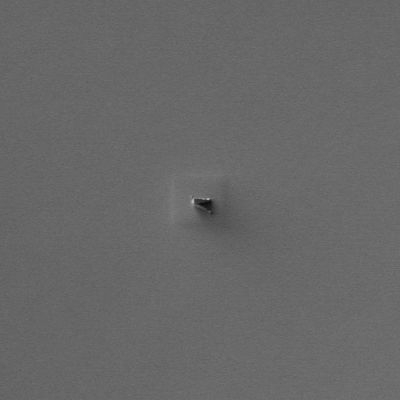
\includegraphics[height=2cm]{defect_1.jpg}};
            % SEM image Class B
            \node[visible on=<3->, line width=0.2mm, draw=white, inner sep=0mm, right=\img of img1] (img2) {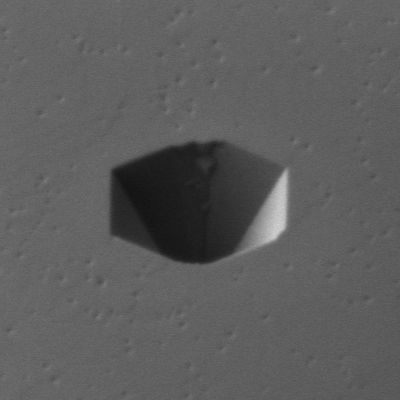
\includegraphics[height=2cm]{defect_2.jpg}};
            % SEM image Class C
            \node[visible on=<3->, line width=0.2mm, draw=white, inner sep=0mm, right=\img of img2] (img3)
            {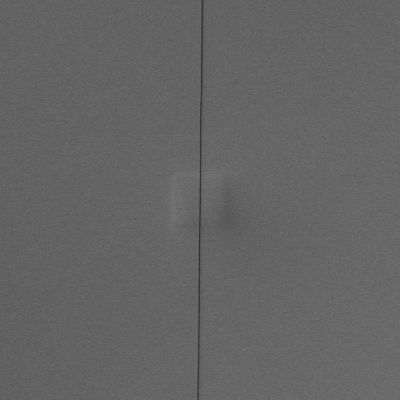
\includegraphics[height=2cm]{defect_3.jpg}};

            % SEM image labels for internal use
            \node[visible on=<4->, above=\adc of img1, text=textfigurecolor, font=\fontsize{10}{24}\selectfont] (class_1)  {Particle};
            \node[visible on=<4->, above=\adc of img2, text=textfigurecolor, font=\fontsize{10}{24}\selectfont] (class_2)  {Pit};
            \node[visible on=<4->, above=\adc of img3, text=textfigurecolor, font=\fontsize{10}{24}\selectfont] (class_3)  {Crack}; 

            % Novelties images box
            \node [visible on=<5->, rectangle, font=\scriptsize, rounded corners, minimum width=2.7cm, minimum height=3.02cm, draw=outlinecolor, fill=outlinecolor, right=\img of sem_tool, xshift = 7.9cm, yshift = 0.32cm] (image_box) {};
            
            % SEM images Novelties
            \node[visible on=<5->, line width=0.2mm, draw=white, inner sep=0mm,right=\imgfinal of img3, xshift = 0.2cm, yshift = 0.2cm] (img6) {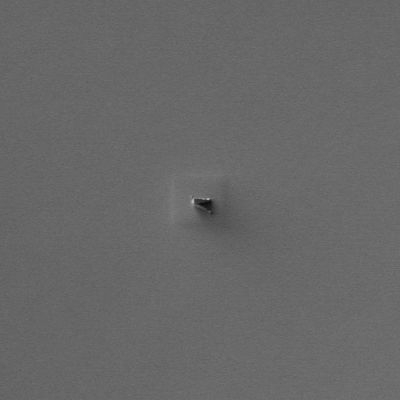
\includegraphics[height=2cm]{defect_4.jpg}};
            \node[visible on=<5->, line width=0.2mm, draw=white, inner sep=0mm,right=\imgfinal of img3, xshift = 0.1cm, yshift = 0.1cm] (img5) {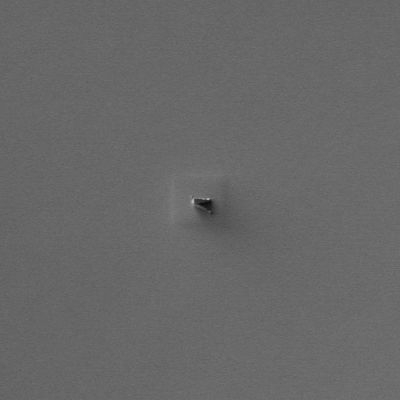
\includegraphics[height=2cm]{defect_4.jpg}};
            \node[visible on=<5->, line width=0.2mm, draw=white, inner sep=0mm,right=\imgfinal of img3] (img4) {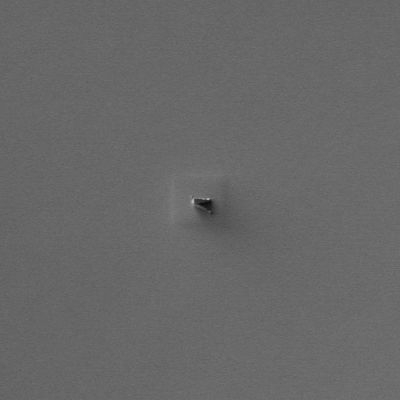
\includegraphics[height=2cm]{defect_4.jpg}};

            % Novelty overlay
            \node [visible on=<5->, novelty] at (img4) {?};

            % SEM image labels for internal and external use
            \node[visible on=<5->, above=\adc of img4, xshift = 0.1cm,  text=textfigurecolor, font=\fontsize{10}{24}\selectfont] (dc_adc_4)  {Novelties};
             
            % Arrow from the image box to the database
            \draw[visible on=<5->, arrow_small]  (10.55,3.95) -- (10.85,3.95);
            
            % Database
            %\node[visible on=<6->, inner sep=0pt,right=\img of img4, xshift = 0.57cm] (database) {
\includegraphics[scale=0.25]{database.png}};
        \end{tikzpicture}
    \end{center}
\end{frame}